\documentclass[aspectratio=169]{beamer}

\usetheme{Madrid} % or your favorite theme
\usecolortheme{default}
\setbeamertemplate{footline}[frame number]
% \setbeamertemplate{navigation symbols}{}

\title[]{Theoretical Spectroscopy via the Cumulant Expansion}
\author[]{Patryk Kozlowski}

\begin{document}

%==================================================
\begin{frame}
  \titlepage
\end{frame}

%==================================================
\begin{frame}{Outline}
  \tableofcontents
\end{frame}

%==================================================
% Add section slides before each section
\AtBeginSection[]{
  \begin{frame}{Outline}
    \tableofcontents[currentsection,hideothersubsections]
  \end{frame}
}

%==================================================
\section{Introduction}

\begin{frame}{X-ray spectroscopy}
\pause
  \begin{itemize}
    \item X-ray spectroscopy is a proven technique for studying materials%Many materials of interest exhibit metallic phases
    \end{itemize}
\pause 
\begin{figure}
  \centering
  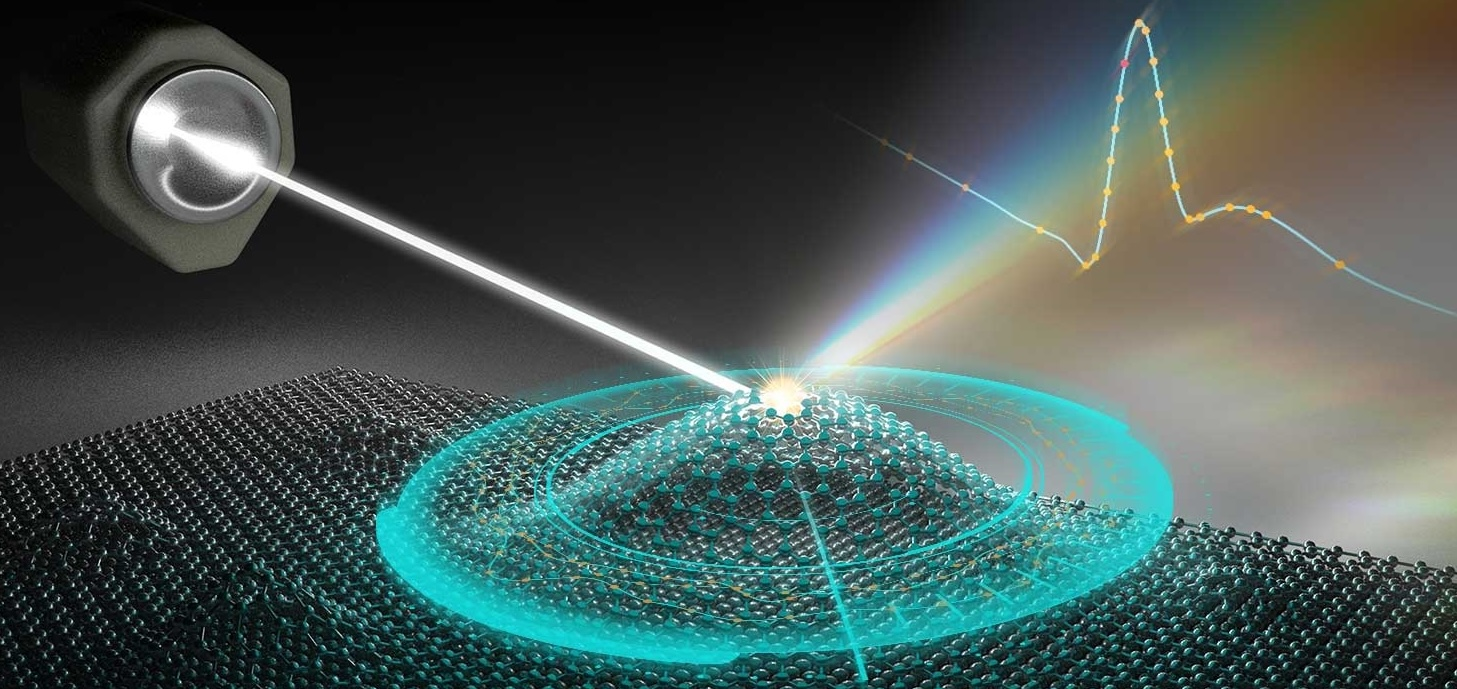
\includegraphics[width=0.8\textwidth]{../figs/Xray_cropped.jpg}
\end{figure}
\pause
\begin{itemize}
    \item The spectral function $A_{pp}(\omega)$ for a core state $p$ is the observable in experiments
  \end{itemize}
\end{frame}
% X-ray spectroscopy is a proven technique for studying materials. Although there are many flavors of X-ray spectroscopy, a common theme throughout is that one shines a beam of X-rays on a sample, exciting core electrons. 
% The spectral function is proportional to the imaginary part of the retarded Green's function of the core state.
\begin{frame}{The uniform electron gas (UEG)}
\pause
%  The UEG as a launchpad for simulating X-ray spectroscopy
\begin{itemize}
\item UEG helps us understand how conduction electrons respond to the creation of a core hole
\pause  
\begin{equation}
\hat{H}_{\mathrm{UEG}}
=
\sum_{\mathbf{K}} \frac{|\mathbf{K}|^2}{2}\, a_{\mathbf{K}}^{\dagger} a_{\mathbf{K}}
\;+\;
\frac{1}{2 \Omega}
\sum_{\mathbf{K}, \mathbf{K}_1, \mathbf{K}_2}
\frac{4 \pi}{|\mathbf{K}|^2}\,
a_{\mathbf{K}_1+\mathbf{K}}^{\dagger}
a_{\mathbf{K}_2-\mathbf{K}}^{\dagger}
a_{\mathbf{K}_2}
a_{\mathbf{K}_1}
\end{equation}
    \pause
      \begin{itemize}
        \item Low density regime\pause$\rightarrow r_s=4$ 
        \pause
        \item Finite supercells\pause$\rightarrow N_{\mathbf{k}} \propto N_e$ \pause $\rightarrow$ Up to $114$ electrons in $485$ orbitals
      \end{itemize}
    \pause
\item I consider several approaches for obtaining $\operatorname{Im}G^R_{pp}(\omega) \propto A_{pp}(\omega)$
\end{itemize}
\end{frame}
% The system I have chosen to study is the uniform electron gas (UEG). The UEG provides an excellent way to build understanding of how conduction electrons screen a core hole, as created in x-ray spectroscopy. The UEG consists of a periodic array of electrons in a neutralizing positive background charge. As in the ab initio case, its Hamiltonian is given by the sum of one-body and two body terms. However, in the UEG the attractive interaction of the electrons with the background is assumed to cancel exactly with the sum of the repulsive self-interaction of the electrons and that of the background.
% Although there are plently of methods which are able to describe the UEG at high density, the low-density regime is more challenging. Here electronic correlation, which is notoriously difficult to solve for, makes a large contribution to the total energy. Therefore, I am interested in simulations of the UEG at a Wigner-Seitz radius of $r_s=4$, which corresponds to the density of metallic sodium.
% When computing spectral properties, the thermodynamic limit value is ultimately of interest. However, this is a computationally intractable problem, so in practice, solid state simulations are done with a finite k-point sampling. There exists a one-to-one mapping between the number of k-points sampled and the number of electrons in a UEG supercell at a fixed density. Therefore, I am interested in simulations of the UEG with a finite number of electrons. In particular, the results I present will be for a UEG supercell with 114 electrons in 485 orbitals.
% therefore, I consider several approaches for obtaining the retarded Green's function for the UEG's core state, which I previously established as the quantity of interest in theoretical X-ray spectroscopy.
\begin{frame}{Cumulant expansion}
\begin{align} G^R_{pp}(t) = G_{0,pp}^R(t) e^{C_{pp}^R(t)}, \label{eq:cumulant_G}\end{align}
\pause where \begin{align} C_{pp}^R(t) = -\frac{1}{\pi}\int d\omega \frac{\mathrm{Im} \Sigma_{pp}^R(\omega)}{\omega^2} \left(e^{-i\omega t} + i \omega t -1\right). \label{eq:cumulant}\end{align}
\pause
\begin{itemize}
  \item This form of the cumulant is the exact solution to the electronic polaron problem \pause
  \item I explore three different approximations for $\Sigma^R_{pp}(\omega)$ : GW, RSPT2, and a size-consistent BWPT2.
\end{itemize}
\end{frame}
% Cumulant is the exact solution to the electronic polaralon problem, which is that of a single core hole coupled to plasmons.
\section{Methods and results}
% \begin{frame}{EOM-CC as an unsatisfactory reference}
% EOM-CC postulates the retarded Green's function as
% \begin{equation}
% G^{R,CC}_{pp}(t) = i \left< \Phi \left| (1+\Lambda) \bar{a^{\dagger}_p}
% e^{i \bar{H}_N t}
% \bar{a}_p \right| \Phi \right>
% \end{equation}
% \pause
% To maintain computational tractability, only EOM-CCSD can be considered.
% \pause
% \begin{figure}
%   \centering
%   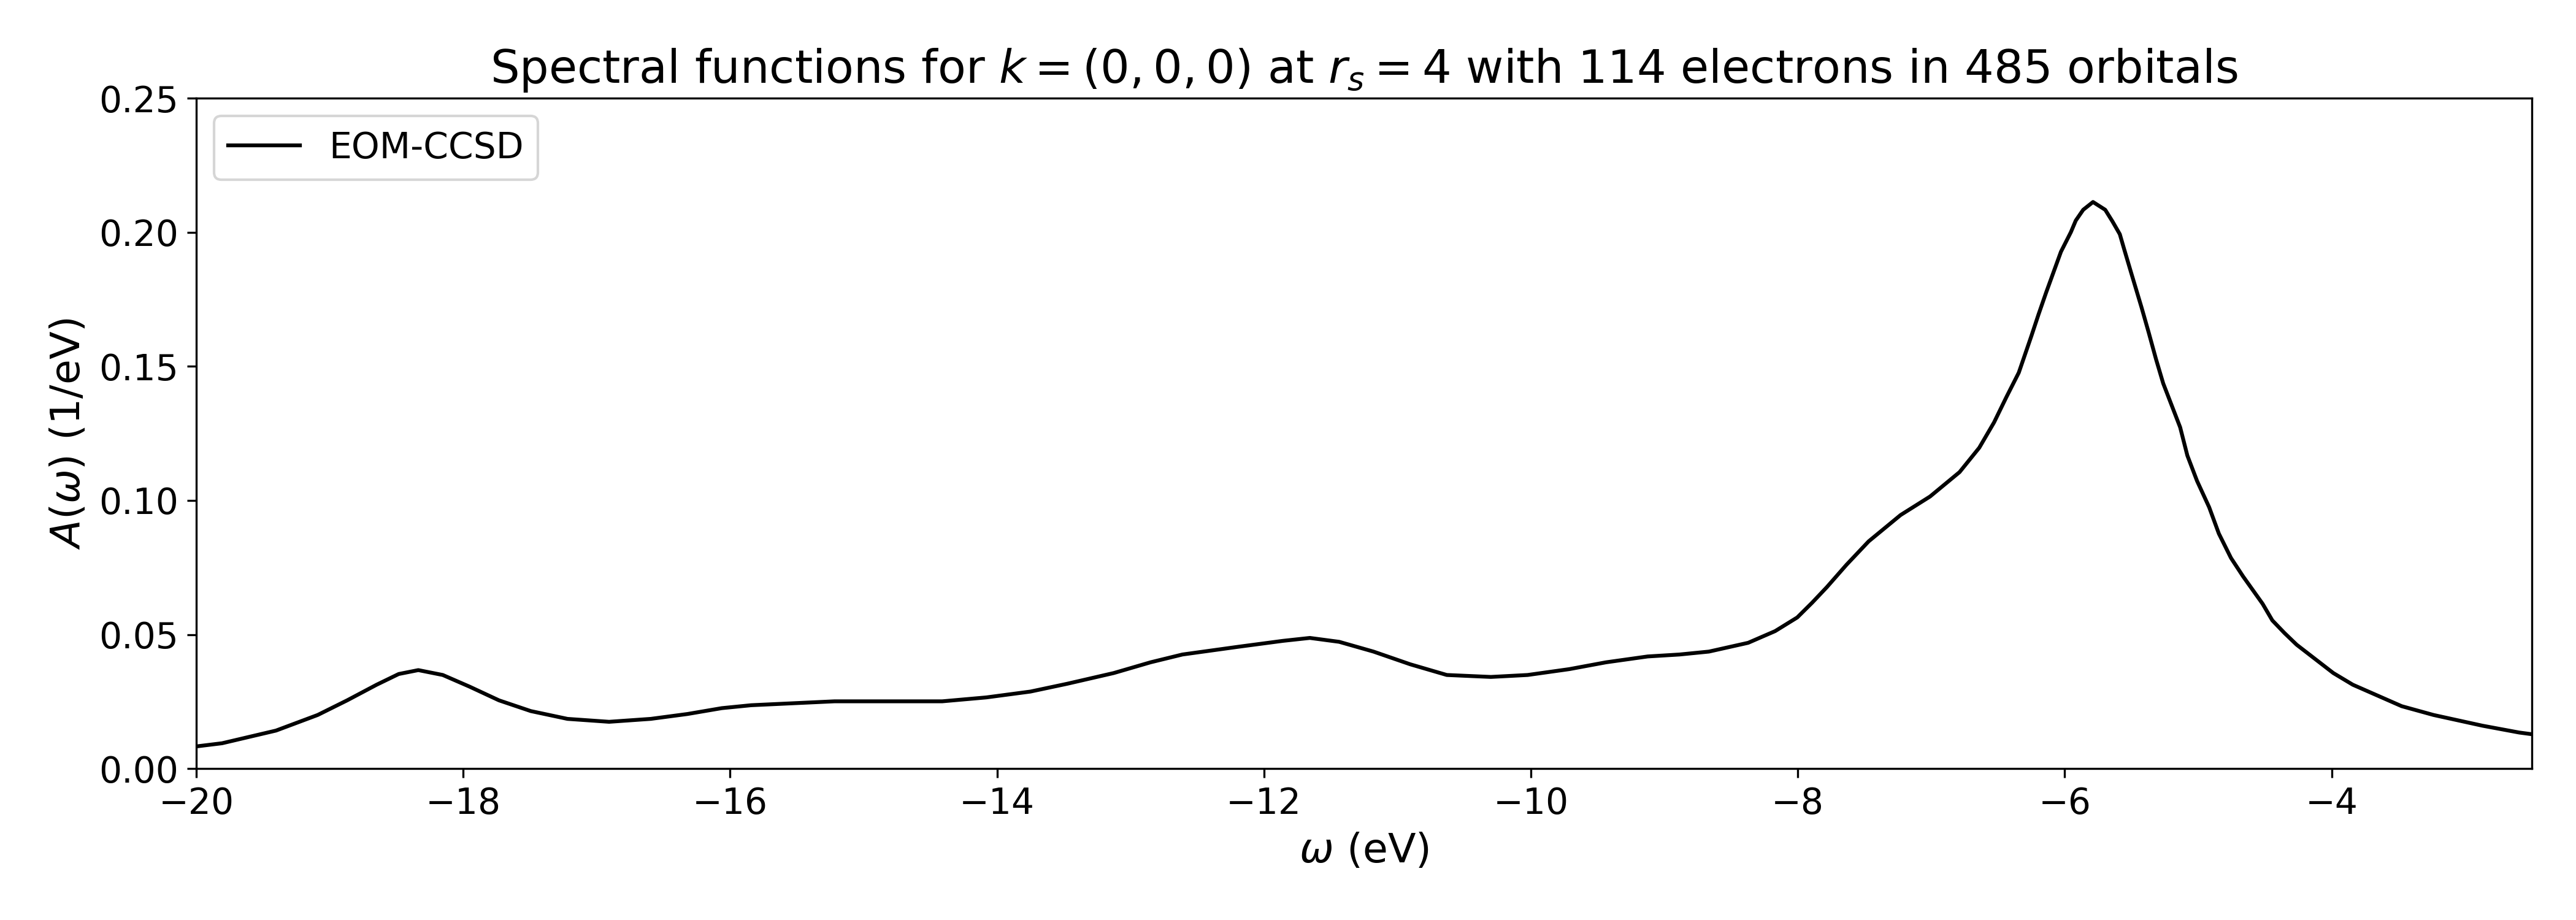
\includegraphics[width=\textwidth]{../figs/v2_bws2_pqe_0.png}
% \end{figure}
% \pause
% \end{frame}
% % EOM-CCSD is nearly exact for small supercells, for larger systems it is inapplicable and its accuracy is unclear.


%==================================================

\begin{frame}{The state of the field: GW+C vs. EOM-CCSD}
\pause

\begin{equation}
  \textcolor{blue}{\Sigma ^{R,GW}_{pp}(\omega )} 
  = G^{R,HF}_{pp}(\omega)^{-1} - G^{R}_{pp}(\omega)^{-1}
\end{equation}

where $\textcolor{blue}{\Sigma^{R,GW}_{pp}}$ is determined via perturbative expansion in the \textcolor{blue}{screened} Coulomb interaction.

\pause
% EOM-CCSD, which only considers single and double excitations, solves for $G^R_{pp}(t)$ as
% \begin{equation}
% G^{R,CC}_{pp}(t) = i \left< \Phi \left| (1+\Lambda) \bar{a^{\dagger}_p}
% e^{i \bar{H}_N t}
% \bar{a}_p \right| \Phi \right>
% \end{equation}
% \pause

\begin{figure}
  \centering
  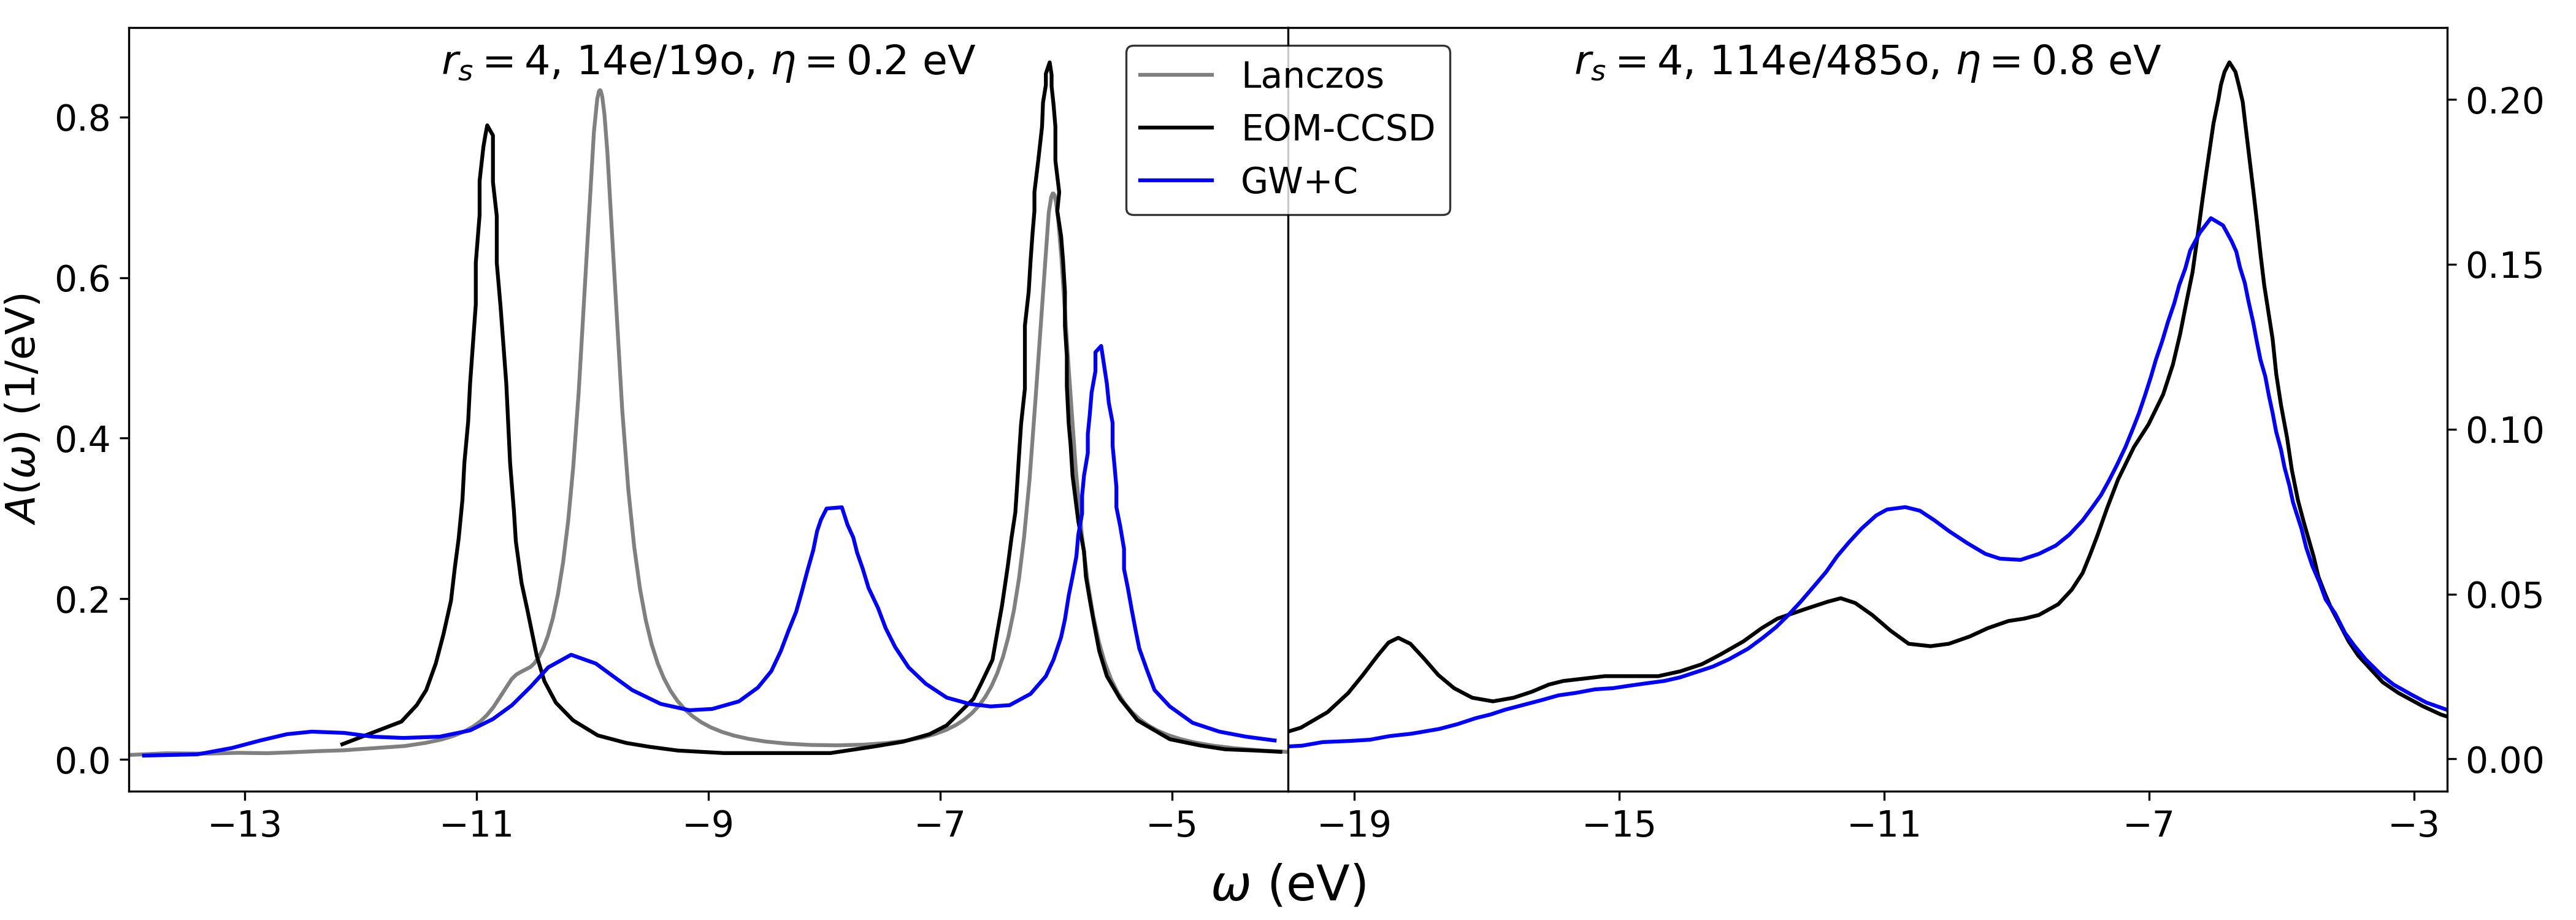
\includegraphics[width=\textwidth]{../figs/two_panel_0.png}
\end{figure}
% GW+C is the state-of-the-art method.
% In particular, the formalism can used to compute core spectral functions analytically in the TDL as was done In the 1980s, when it was shown to accurately reproduce core spectra of simple alkali metals. 
% However, GW+C spectral function diverges from EOM-CCSD at small system sizes, where we know the latter is nearly exact. As can be seen, for the intermediate size supercell I consider, this is again the case, which is a cause for concern. Therefore, one would want a third opinion.
\end{frame}
\begin{frame}{A poor choice: RSPT2+C}
\pause
\begin{equation}
  \textcolor{red}{\Sigma ^{R,(2)}_{pp}(\omega )} = G^{R,HF}_{pp}(\omega)^{-1} - G^{R}_{pp}(\omega)^{-1}
\end{equation}
where $\textcolor{red}{\Sigma^{R,(2)}_{pp}}$ is determined via perturbative expansion in the \textcolor{red}{bare} Coulomb interaction.
\pause
\begin{figure}
  \centering
  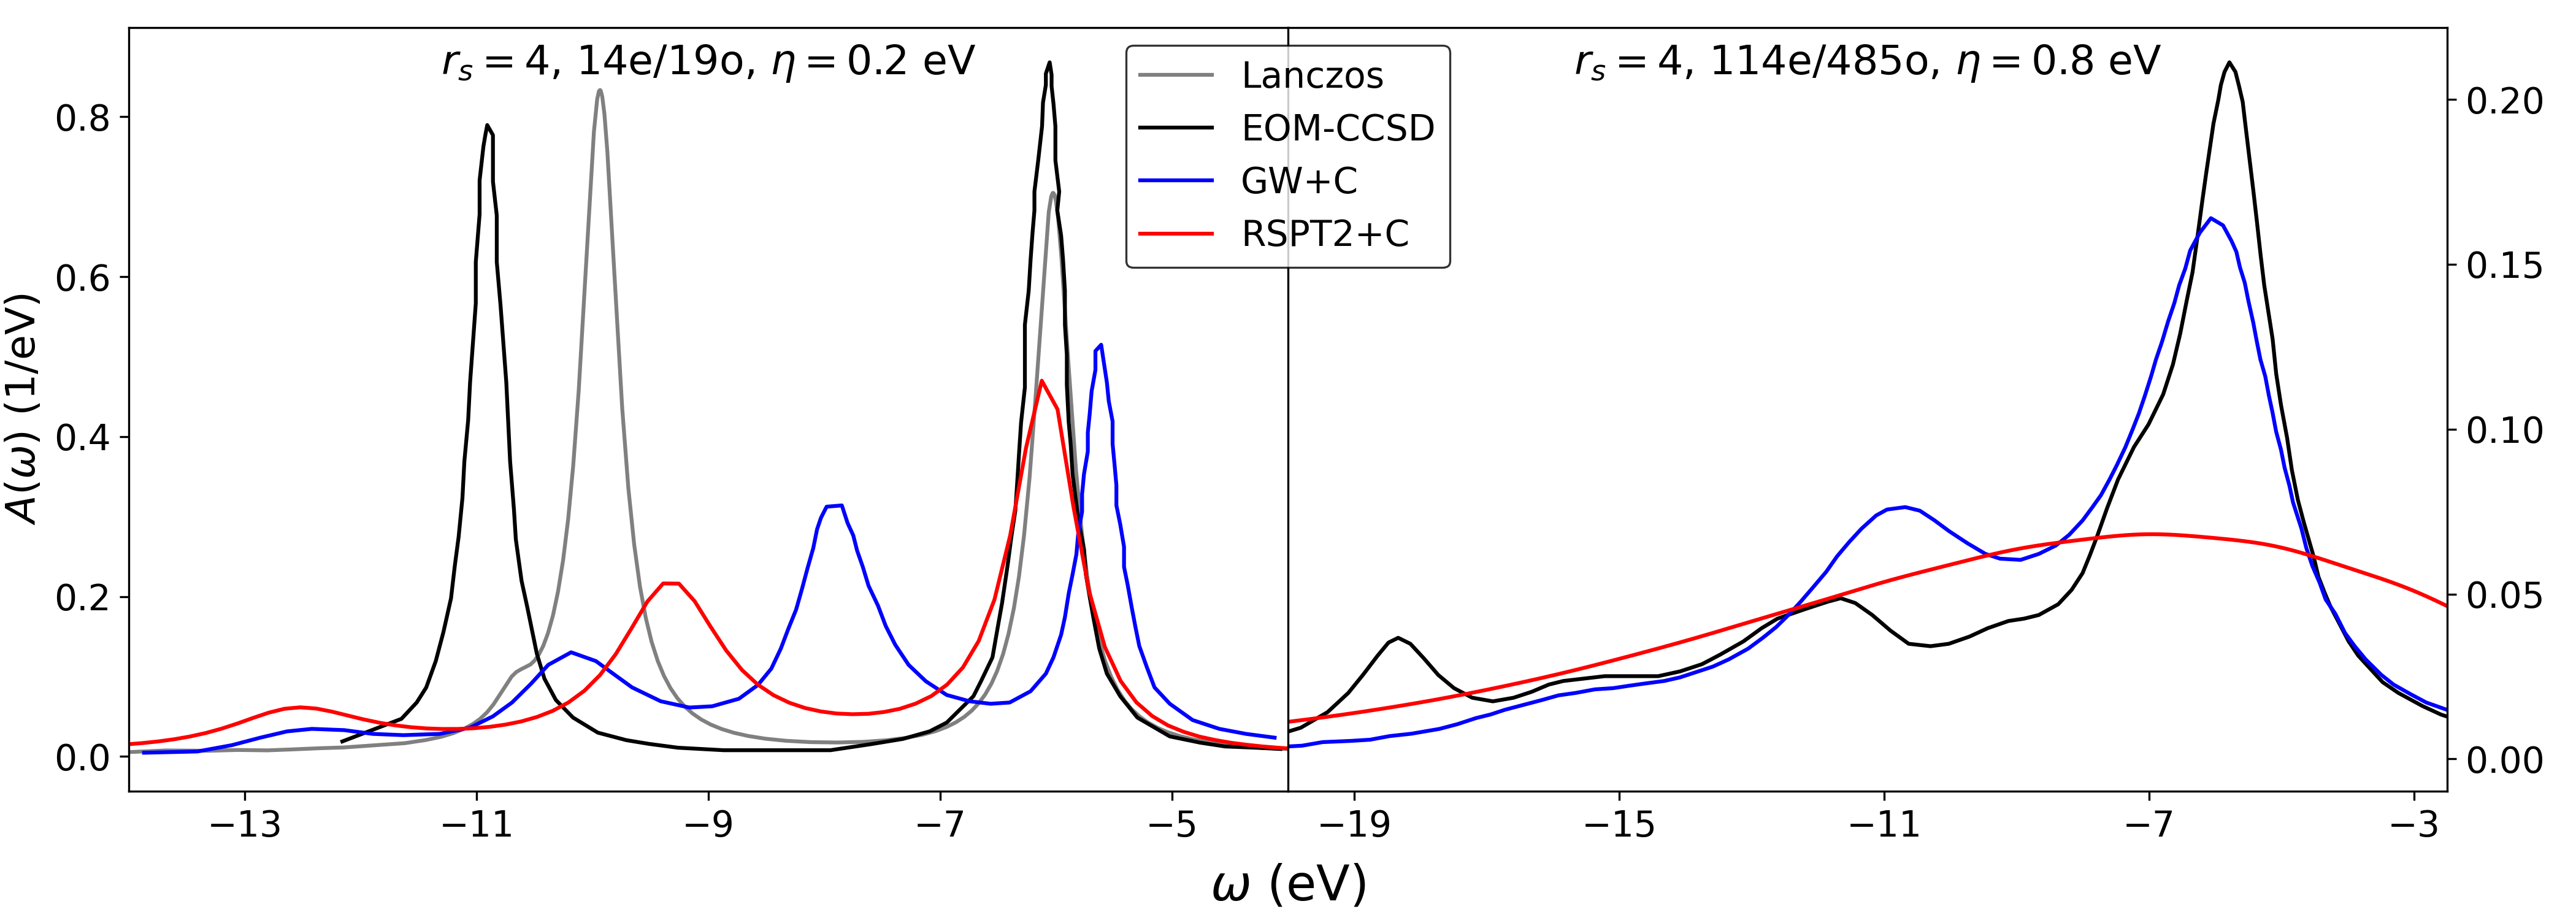
\includegraphics[width=\textwidth]{../figs/two_panel_1.png}
\end{figure}
\end{frame}
% A natural choice would lie within second order perturbation theory (PT2), but as we will soon see, this is a poor choice.
% This can be understood because we know PT2 diverges for metallic systems, like the UEG.
\begin{frame}{A promising choice: BWs2+C}
\pause 
\begin{equation}
  \textcolor{green}{\Sigma ^{R,\text{BWs2}}_{pp}(\omega )} = \textcolor{green}{G^{R,\text{BWs2}}_{pp}(\omega)^{-1}} - G^{R}_{pp}(\omega)^{-1}
\end{equation}
where $\textcolor{green}{\Sigma^{R,\text{BWs2}}_{pp}}$ is determined via perturbative expansion in the \textcolor{red}{bare} $V$, but is now \textcolor{blue}{screened}
\pause
\begin{figure}
  \centering
  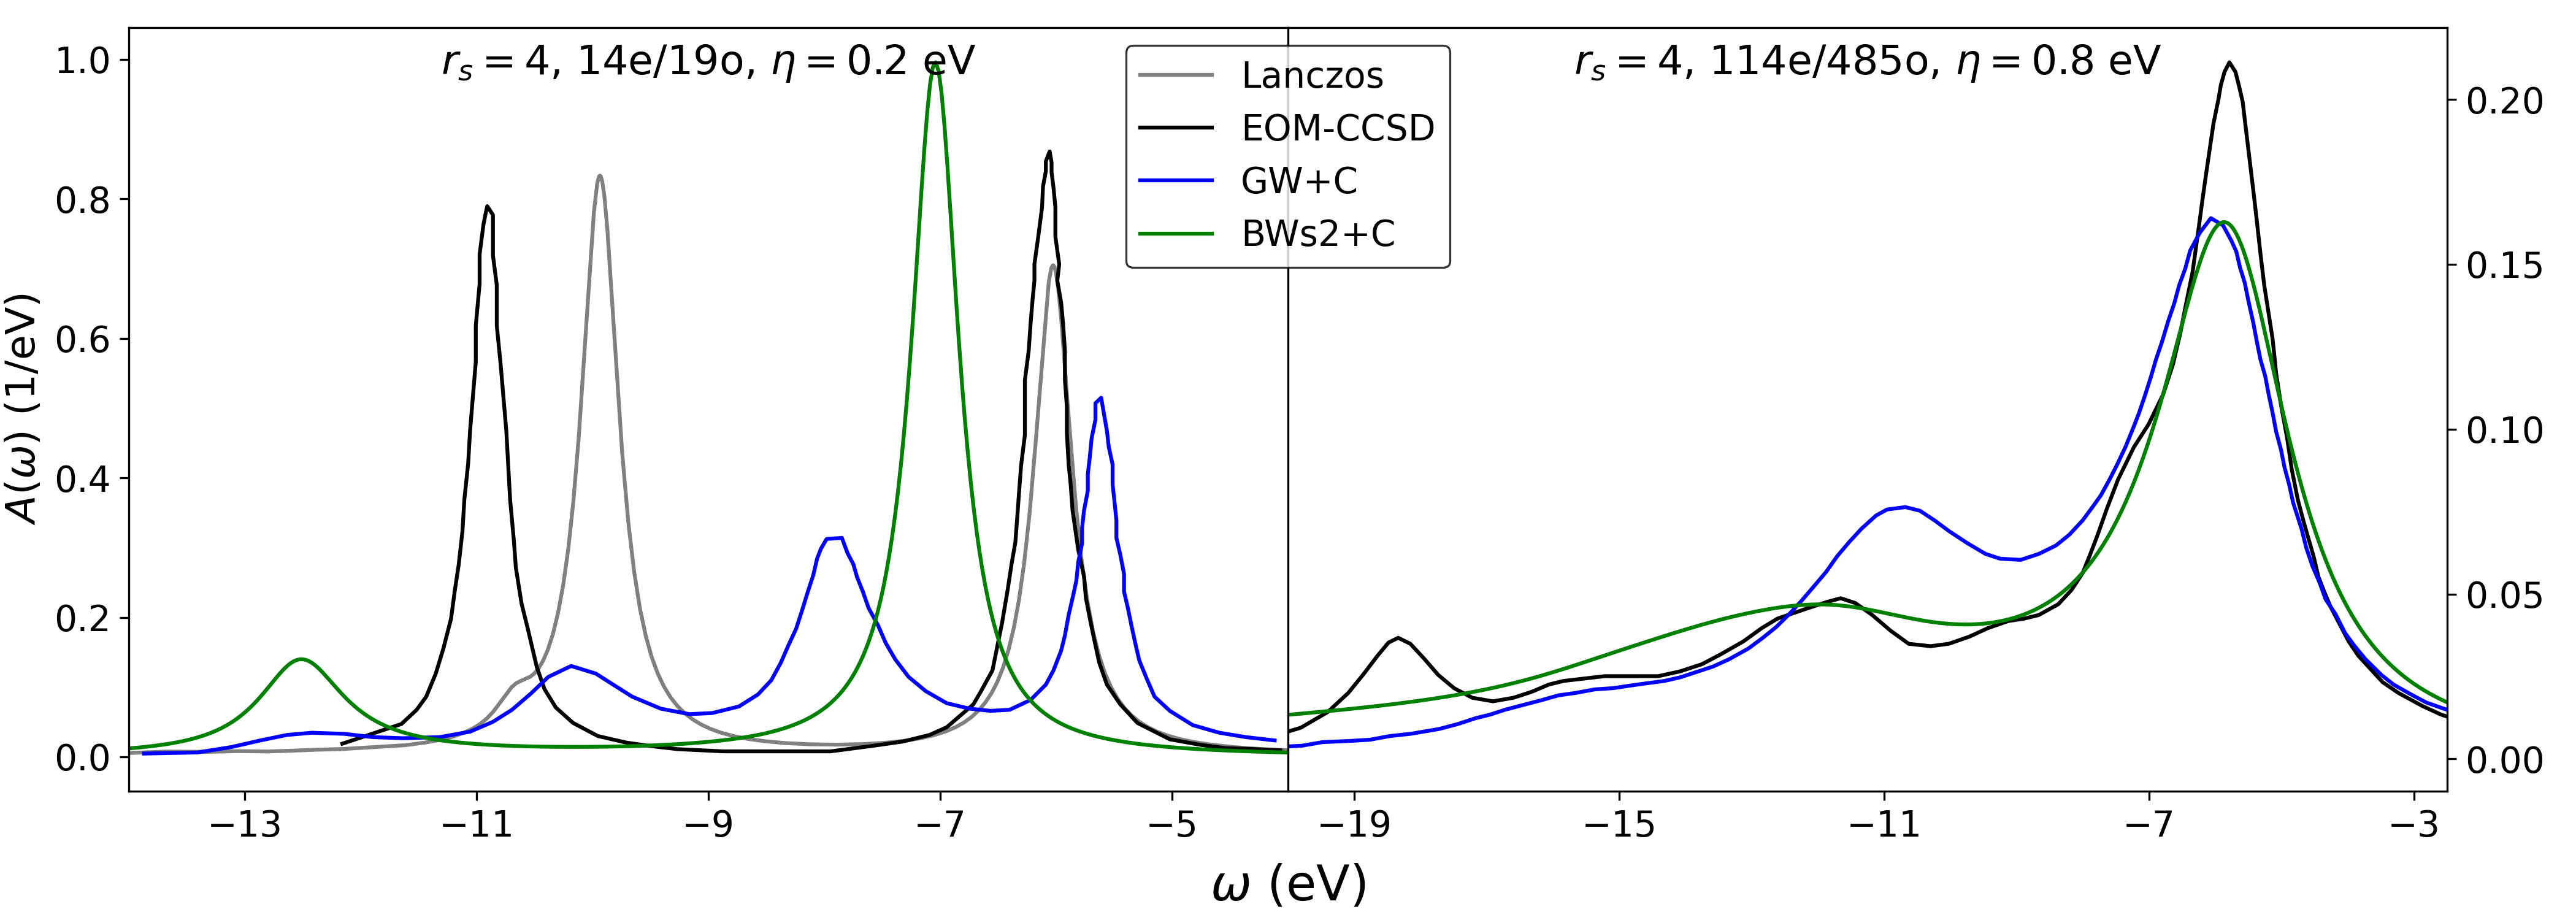
\includegraphics[width=\textwidth]{../figs/two_panel_2.png}
\end{figure}
\end{frame}
% Brillouin-Wigner perturbation theory not gotten much interest in the past, due to a lack of size-consistency. Recently, Head-Gordon and co-workers propose a size-consistent second-order Brillouin-Wigner perturbation theory, which they call BWs2, and it has been demonstrated to accurately compute ground-state properties of metals. One of my labmates was able to show that BWs2 admits a self-energy that satisfies the Dyson equation. This motivated me to derive a BWs2 cumulant.


%==================================================
\section{Future directions}

\begin{frame}{Self-consistent cumulant}
GW+C has an unsatisfactory dependence on the choice of the starting point. 
\pause
\begin{enumerate}
\item Solve for the Green's function via
\begin{align} G^R_{pp}(t) = G_{0,pp}^R(t) e^{C_{pp}^R(t)} \label{eq:cumulant_G}\end{align}
using the cumulant as \begin{align} C_{pp}^R(t) = -\frac{1}{\pi}\int d\omega \frac{\mathrm{Im} \Sigma_{pp}^R(\omega)}{\omega^2} \left(e^{-i\omega t} + i \omega t -1\right) \label{eq:cumulant}\end{align}
\pause
\item Solve for a new self-energy via the below definition and plug back into equation~\ref{eq:cumulant}
\begin{equation}
\Sigma^R_{pp}(\omega ) = \left[G_{0,pp}^R(\omega)\right]^{-1} - \left[G^R_{pp}(\omega)\right]^{-1} \label{eq:rearranged_dyson}
\end{equation}
\pause
\item Iterate until self-consistency
\end{enumerate}
\end{frame}
% Another known limitation of the state-of-the-art GW+C approach is that it is heavily dependent on the choice of the starting point. A potential solution to this problem is to solve for the cumulant self-consistently. There have only been a few studies of the self-consistent cumulant in the literature and these all perform the self-consistency analytically in the TDL. Given my interest in finite supercells, I want to pursue self-consistency numerically. The scheme I have in mind is as follows.
\begin{frame}
  \centering
  \Large Questions?
\end{frame}
\begin{frame}{BWs2 theory}
  PT2 splits the Hamiltonian into a zeroth order part, $\hat{H}^{(0)}$, and a perturbation, $\hat{V}$, as
\begin{equation}
  \hat{H} = \hat{H}^{(0)} + \hat{V}.
\end{equation}
The Moller-Plesset partitioning takes
\begin{equation}
  \hat{H}^{(0)}=f_{pq} \hat{a}_p^{\dagger} \hat{a}_q,
\end{equation}
where $f_{pq}$ is the Fock matrix. In contrast, the size-consistent Brillouin-Wigner partitioning takes\cite{Dittmer2025-rw}
\begin{equation}
  \hat{H}^{(0)}=f_{pq} \hat{a}_p^{\dagger} \hat{a}_q+\frac{\alpha_1}{8}\left(t_{i k}^{a b(1)}\langle j k \| a b\rangle+t_{j k}^{a b(1)}\langle i k \| a b\rangle-\frac{2}{N} t_{k l}^{a b(1)}\langle k l \| a b\rangle \delta_{i j}\right) \hat{a}_i^{\dagger} \hat{a}_j +\frac{\alpha _2}{8}\left(t_{i j}^{a c(1)}\langle i j \| b c\rangle+t_{i j}^{b c}{ }^{(1)}\langle i j \| a c\rangle\right) \hat{a}_a^{\dagger} \hat{a}_b,
\end{equation}
where $t^{(1)}$ are the doubles amplitudes of the perturbation theory to first order and $\alpha_1$ and $\alpha _2$ are empirical parameters.
\end{frame}
\begin{frame}{Cumulant formulations}
\begin{enumerate}
  \item GW cumulant
  \begin{align}
    C_{pp}^{R,\mathrm{GW}}(t) 
      &= \sum_{i\nu} \zeta_{pi\nu} \left[ e^{-i\Delta_{pi\nu} t} - 1 + i\Delta_{pi\nu} t \right] 
       + \sum_{a\nu} \zeta_{pa\nu} \left[ e^{-i\Delta_{pa\nu} t} - 1 + i\Delta_{pa\nu} t \right]
  \end{align}
  where $\zeta_{pi\nu} = \left(\frac{M_{pi\nu}}{\Delta_{pi\nu}}\right)^2\quad,\quad\Delta_{pi\nu} = \epsilon_p - \epsilon_i + \omega_\nu$ and $\zeta_{pa\nu} = \left(\frac{M_{pa\nu}}{\Delta_{pa\nu}}\right)^2 \quad,\quad\Delta_{pa\nu} = \epsilon_p - \epsilon_a - \omega_\nu$.

  \item Second-order cumulant
  \begin{align}
    C_{pp}^{(2)}(t) 
      &= \frac{1}{2}\sum_{iab} \frac{\left< pi \left| \right| ab \right>^2}{\left(\epsilon_{pi}^{ab}\right)^2}
\left(e^{-i \epsilon_{pi}^{ab} t} +i \epsilon_{pi}^{ab} t -1 \right)
+\frac{1}{2}\sum_{ija} \frac{\left< pa \left| \right| ij \right>^2}{\left(\epsilon_{pa}^{ij}\right)^2}
\left(e^{-i \epsilon_{pa}^{ij} t} +i \epsilon_{pa}^{ij} t -1 \right) 
  \end{align}
  where
  \[
    \epsilon_{pi}^{ab} = \epsilon_{a}+\epsilon_{b}-\epsilon_{p}-\epsilon_{i},
    \qquad
    \epsilon_{pa}^{ij} = \epsilon_{i}+\epsilon_{j}-\epsilon_{p}-\epsilon_{a}.
  \]

\end{enumerate}
\end{frame}
\begin{frame}{Cumulant formulations (continued)}
\begin{enumerate}
\item BWs2 cumulant
  \begin{equation}
    C_{pp}^{\mathrm{BWs2}}(t) = 
    \frac{1}{2} \sum_{i a b}\frac{\langle p i \| a b\rangle^2 }{\left(\tilde{\varepsilon}_{p i}^{a b}\right)^2}
      \left(e^{-i \tilde{\varepsilon}_{p i}^{a b} t} + i \tilde{\varepsilon}_{p i}^{a b} t -1 \right) 
    + \frac{1}{2}\sum_{i j a} \frac{\langle p a \| i j\rangle^2}{\left(\tilde{\varepsilon}_{p a}^{i j}\right)^2} 
      \left(e^{-i \tilde{\varepsilon}_{p a}^{i j} t} - 1 \right),
  \end{equation}
  where
  \[
    \tilde{\varepsilon}_{p i}^{a b} = \tilde{\epsilon}_p - \tilde{\epsilon}_i + \tilde{\epsilon}_a - \tilde{\epsilon}_b,
    \qquad
    \tilde{\varepsilon}_{p a}^{i j} = \tilde{\epsilon}_p + \tilde{\epsilon}_a - \tilde{\epsilon}_i - \tilde{\epsilon}_j.
  \]
\end{enumerate}
\end{frame}

\begin{frame}{Dyson equation rearrangement}
\small
Start from the definition of the retarded self-energy
\begin{equation}
  \Sigma^R_{pp}(\omega) 
  = \bigl[G_{0,pp}^R(\omega)\bigr]^{-1} 
  - \bigl[G_{pp}^R(\omega)\bigr]^{-1} \,.
\end{equation}
We can rearrange to get
\begin{equation}
  \bigl[G_{pp}^R(\omega)\bigr]^{-1}
  = \bigl[G_{0,pp}^R(\omega)\bigr]^{-1} - \Sigma^R_{pp}(\omega)
  \quad\Longleftrightarrow\quad
  G^R = G_0^R + G_0^R \Sigma^R G^R \,.
\end{equation}
Expanding to first order in the interaction $V$ gives
\begin{equation}
  G^R = G_0^R + G_0^R \Sigma^R G_0^R + \mathcal{O}(V^2)\,.
\end{equation}
\end{frame}

\end{document}